\documentclass[border=10pt]{standalone}
\usepackage{tikz}
\usetikzlibrary{arrows.meta, calc}   % ← 关键：calc 不能少
\definecolor{inFill}{RGB}{183,224,177}
\definecolor{inLine}{RGB}{32,102,32}
\definecolor{hidFill}{RGB}{199,203,243}
\definecolor{hidLine}{RGB}{52,58,143}
\definecolor{outFill}{RGB}{243,199,199}
\definecolor{outLine}{RGB}{143,52,52}
\definecolor{lineC}{RGB}{38,44,110}
\begin{document}
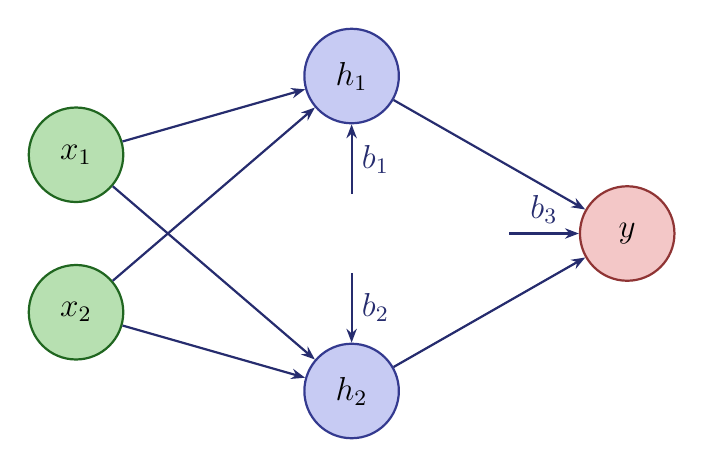
\begin{tikzpicture}[
    >={Stealth[length=5pt]}, line width=0.8pt, font=\large,
    inp/.style={circle, draw=inLine, fill=inFill, minimum size=1.2cm, inner sep=0pt},
    hid/.style={circle, draw=hidLine, fill=hidFill, minimum size=1.2cm, inner sep=0pt},
    outp/.style={circle, draw=outLine, fill=outFill, minimum size=1.2cm, inner sep=0pt},
    arr/.style={lineC, ->},
  ]
  % 节点
  \node[inp]  (x1) at (0, 1)   {$x_1$};
  \node[inp]  (x2) at (0,-1)   {$x_2$};
  \node[hid]  (h1) at (3.5, 2) {$h_1$};
  \node[hid]  (h2) at (3.5,-2) {$h_2$};
  \node[outp] (y)  at (7, 0)   {$y$};

  % 全连接箭头
  \foreach \i in {x1,x2}
    \foreach \j in {h1,h2}
      \draw[arr] (\i) -- (\j);
  \draw[arr] (h1) -- (y);
  \draw[arr] (h2) -- (y);

  % 偏置箭头：绝对坐标起点，方向平行于 $h_1/h_2 \to y$
  % 几何计算：终点坐标和方向角度
  % h1->y 向量方向 (3.5, -2), dist dist(h1,y)=4.03, angle approx -29.7 degrees.
  % b1 终点 (h1), 起点从西北方向沿反向平行于 h1->y 的 $1.5$cm.
  % 起点 = (3.5, 2) + 0.372*(-3.5, 2) = (3.5, 2) + (-1.3, 0.74) = (2.2, 2.74).

  % h2->y 向量方向 (3.5, 2), dist dist(h2,y)=4.03, angle approx 29.7 degrees.
  % b2 终点 (h2), 起点从西南方向沿反向平行于 h2->y 的 $1.5$cm.
  % 起点 = (3.5, -2) + 0.372*(-3.5, -2) = (3.5, -2) + (-1.3, -0.74) = (2.2, -2.74).

  % b3 终点 (y), 从左边斜着来，角度和 h1->y 或 h2->y 角度一致。
  % 为了视觉对称和满足“左边斜着”，我将使用从左下方斜向上的，斜度和 b2 反向平行（西南）。
  % 终点 (7, 0), 起点从西南方向移动 $1.5$cm.
  % 起点 = (7, 0) + 0.372*(-3.5, -2) = (7, 0) + (-1.3, -0.74) = (5.7, -0.74).

  % tikz 自动缩短到节点边界
  \draw[arr] (3.5, 0.5)  -- (h1) node[midway, right] {$b_1$};   % 正下方 → 竖直向上指 h1
  \draw[arr] (3.5,-0.5)  -- (h2) node[midway, right] {$b_2$};   % 正上方 → 竖直向下指 h2
  \draw[arr] (5.5, 0) -- (y) node[midway, above] {$b_3$};       % 不变：水平指 y，居中  \draw[arr] (5.5, 0) -- (y) node[midway, above] {$b_3$};   % 沿 x 轴水平指 y，正好在两根斜线正中间
  
\end{tikzpicture}
\end{document}